\documentclass{article}

% if you need to pass options to natbib, use, e.g.:
%     \PassOptionsToPackage{numbers, compress}{natbib}
% before loading neurips_2019

% ready for submission
% \usepackage{neurips_2019}

% to compile a preprint version, e.g., for submission to arXiv, add add the
% [preprint] option:
%     \usepackage[preprint]{neurips_2019}

% to compile a camera-ready version, add the [final] option, e.g.:
     \usepackage[preprint]{neurips_2019}

% to avoid loading the natbib package, add option nonatbib:
%     \usepackage[nonatbib]{neurips_2019}

\usepackage[utf8]{inputenc} % allow utf-8 input
\usepackage[T1]{fontenc}    % use 8-bit T1 fonts
\usepackage{hyperref}       % hyperlinks
\usepackage{url}            % simple URL typesetting
\usepackage{booktabs}       % professional-quality tables
\usepackage{amsfonts}       % blackboard math symbols
\usepackage{nicefrac}       % compact symbols for 1/2, etc.
\usepackage{microtype}      % microtypography
\usepackage{graphicx}
\usepackage{subcaption}
\captionsetup{compatibility=false}
\usepackage{float}
\usepackage{url}



\title{Deep Learning Papers Review: Striving for Simplicity in Off-policy Deep Reinforcement Learning}

% The \author macro works with any number of authors. There are two commands
% used to separate the names and addresses of multiple authors: \And and \AND.
%
% Using \And between authors leaves it to LaTeX to determine where to break the
% lines. Using \AND forces a line break at that point. So, if LaTeX puts 3 of 4
% authors names on the first line, and the last on the second line, try using
% \AND instead of \And before the third author name.

\author{%
  Seungwon Kim\\
  Incheon International Airport Corporation\\
  Georgia Institute of Technology\\
  \texttt{skim3222@gatech.edu} \\
  % examples of more authors
  % \And
  % Coauthor \\
  % Affiliation \\
  % Address \\
  % \texttt{email} \\
  % \AND
  % Coauthor \\
  % Affiliation \\
  % Address \\
  % \texttt{email} \\
  % \And
  % Coauthor \\
  % Affiliation \\
  % Address \\
  % \texttt{email} \\
  % \And
  % Coauthor \\
  % Affiliation \\
  % Address \\
  % \texttt{email} \\
}

\begin{document}

\maketitle

\section{Background}

Off-policy Q-learning allows two different policies: behavior policy and target policy. As in figure 1, behavior policy selects an action, whereas the target policy is used to estimate the next state-action value. On the other hand, on-policy learning uses the same policy for choosing the action to execute and estimating the next state-action value. Additionally, the term off-policy can be used to indicate pure exploratory random behavior, which is literally off from the current policy, whereas on-policy can suggest following current policy, which means acting greedily or choosing the action using epsilon-greedy strategy.

\begin{figure}[H]
  \centering
    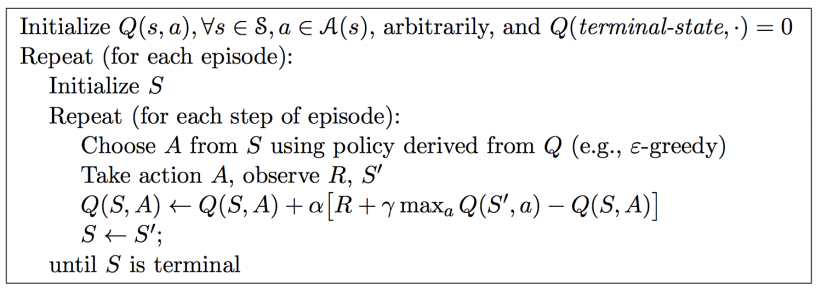
\includegraphics[width=0.6\linewidth]{0.png}
  \caption{Off-policy Q-learning}
\end{figure}

Deep Q-learning (DQN) algorithm is labeled as off-policy RL algorithm but it is considered as “online” rather than “offline” since it exploits near on-policy behavior such as epsilon-greedy with an experience replay. Training DQN in offline setting, i.e. batch setting, which means using data that have been already logged, doesn’t work well due to the extrapolation error.

\begin{figure}[H]
  \centering
    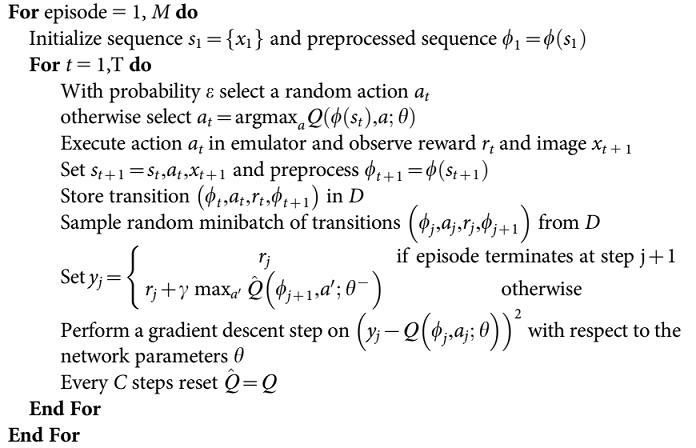
\includegraphics[width=0.5\linewidth]{0_1.png}
  \caption{DQN in online setting}
\end{figure}

Off-policy RL algorithms such as Q-learning are more practical and efficient to handle real-world problems with already logged data than on-policy algorithms such as policy gradient since in principle, off-policy algorithm can learn from any data collected by any policy. But off-policy RL algorithms are unstable and there is no guarantee that it converges especially when using neural networks for function approximation.

To make stable off-policy DQN, here have been various advances (see figure 3) such as distributional RL: C51 or quantile regression DQN (QR-DQN). Both C51 and QR-DQN obatin state-of-the-art performance on Atrai 2600 games by estimating the distribution of return using support with assigned probabilities rather than estimating expected return.

\begin{figure}[H]
  \centering
    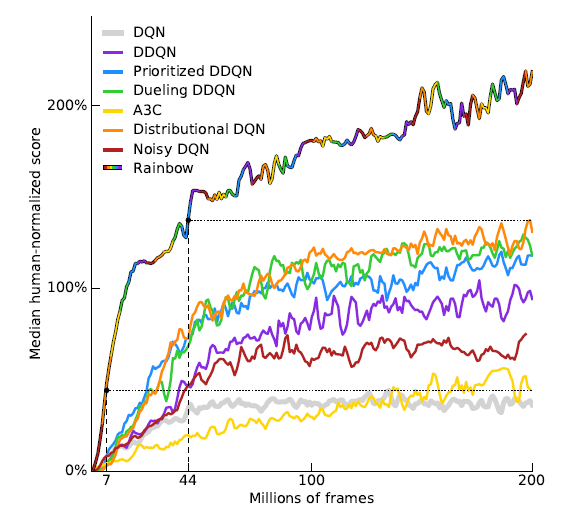
\includegraphics[width=0.4\linewidth]{0_2.png}
  \caption{Rainbow DQN}
\end{figure}

\section{Main point, Summary of this paper}

This paper investigates training DQN with the batch setting, i.e. “ Is it possible to make successful agents using completely on offline logged data?” It presents the performance of distributional RL, nature DQN(2015 Mnih et al) on Atrai 2600 games in both batch setting(offline setting) and online setting. Surprisingly, offline QR-DQN outperforms online C51 and online DQN, which is contrary to recent work.

This paper also tries to make RL algorithms as simple as possible. In spite of recent advances in DQN, those might lead to complex hypothesis and it is more likely to coincidentally fits data than simple hypothesis does (Occam’s razor). It is important to ask “ Are those advances really necessary? “ The paper proposes Ensemble DQN and Random Ensemble Mixture (REM) DQN, which are way simpler than distributional RL, and it shows that REM DQN outperforms C51 and QR-DQN in the offline setting and online REM DQN performs comparably with online QR-DQN.

\section{Proposed Architecture}

\begin{figure}[H]
  \centering
    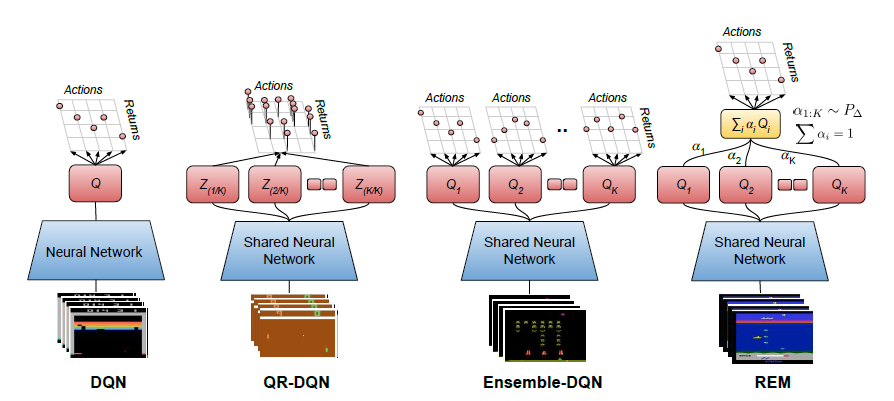
\includegraphics[width=0.5\linewidth]{arch.png}
  \caption{Architecutre}
\end{figure}

DQN, QR-DQN, Ensemble-DQN, and REM DQN use the same network architecture but DQN outputs state-action value Q(s,a) and QR-DQN outputs K *|A| number of Z to represent the distribution of return rather than just estimating the expected value of the return. Ensemble-DQN is a simple extension of DQN, which uses an ensemble of Q(s,a) (see below). Each random Q-head with its target is used to compute Bellman error respectively as shown in below loss function.

REM-DQN uses a convex combination of Q values to estimate Q-values (see below). Each coefficient alpha is randomly drawn from a categorical distribution.

\section{Experiments}
Experiments are performed with the same number of Q-heads at 200 and the same value of other parameters. Experience replay consists of 50 million tuples of (observation, action, reward, next observation), which have been logged by Nature DQN(Mnih et al 2015). Offline QR-DQN outperforms online C51 and online DQN. REM DQN outperforms C51 and QR-DQN in the offline setting and online REM DQN performs comparably with online QR-DQN.


\begin{figure}[H]
  \centering
    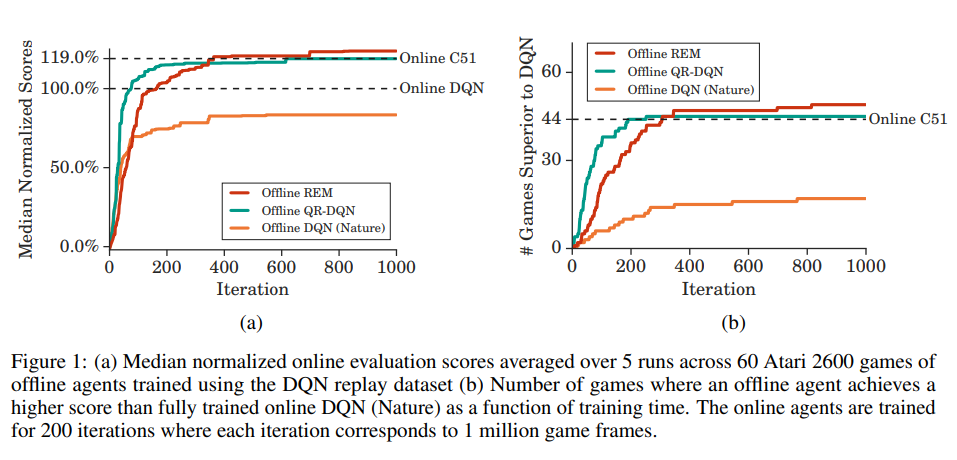
\includegraphics[width=0.6\linewidth]{3.png}
\end{figure}

\begin{figure}[H]
  \centering
    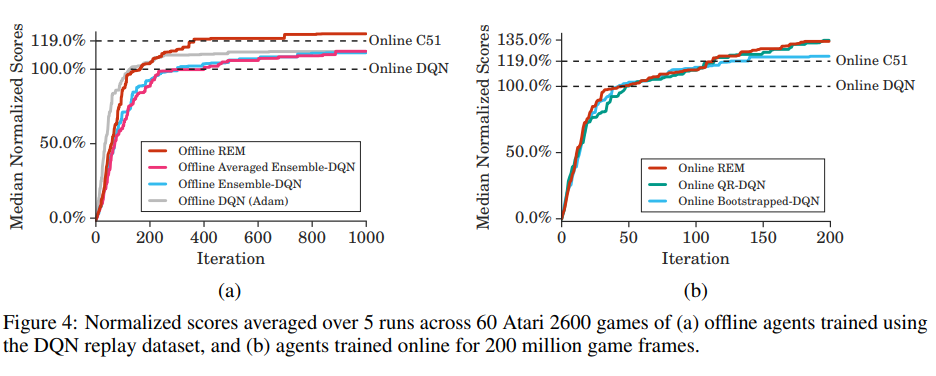
\includegraphics[width=0.6\linewidth]{3_2.png}
\end{figure}


\begin{figure}[H]
  \centering
    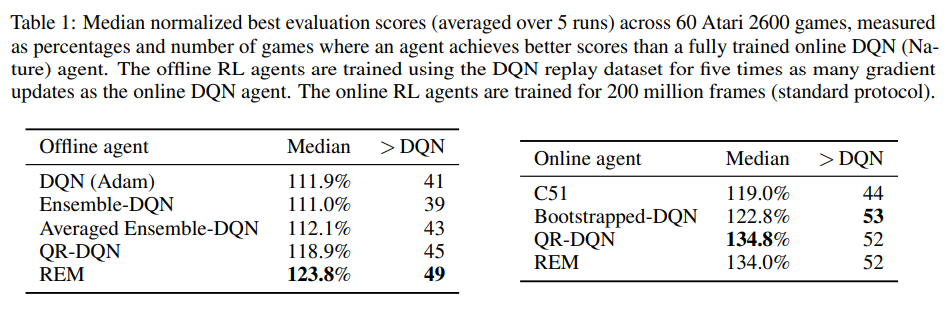
\includegraphics[width=0.6\linewidth]{3_3.png}
\end{figure}

\section{Contribution}
This paper shows that it is possible to successfully train DQN in batch setting, which uses a fixed dataset without interacting with environments. Using a common logged dataset can improve the reproducibility of off-policy RL algorithms, accelerating research by serving a testbed similar to Imagenet dataset in computer vision.

\bibliographystyle{plain}
\bibliography{refs}

\end{document}

